% 第 2 章：图的形状（图论总览）。素材：blog advanced/graph-shapes.md；思维导图和题型表由同一份数据生成
\section{图的形状：环相关的题先看这张图}

第 3、4、5 章都和环有关：判环、函数图、建图。三章各讲一种问法或一种输入，放在一起容易乱。
这一章先给一张总图：\textbf{先按整张图的方向和出度选一支，再按每个连通块的边数或有向环定形状}。
形状定了，每块有几个环、剥叶子剩下什么、该拿哪个工具也就定了；后面三章是其中几片叶子的细节。

\subsection{总览：两步定形状}

\begin{center}
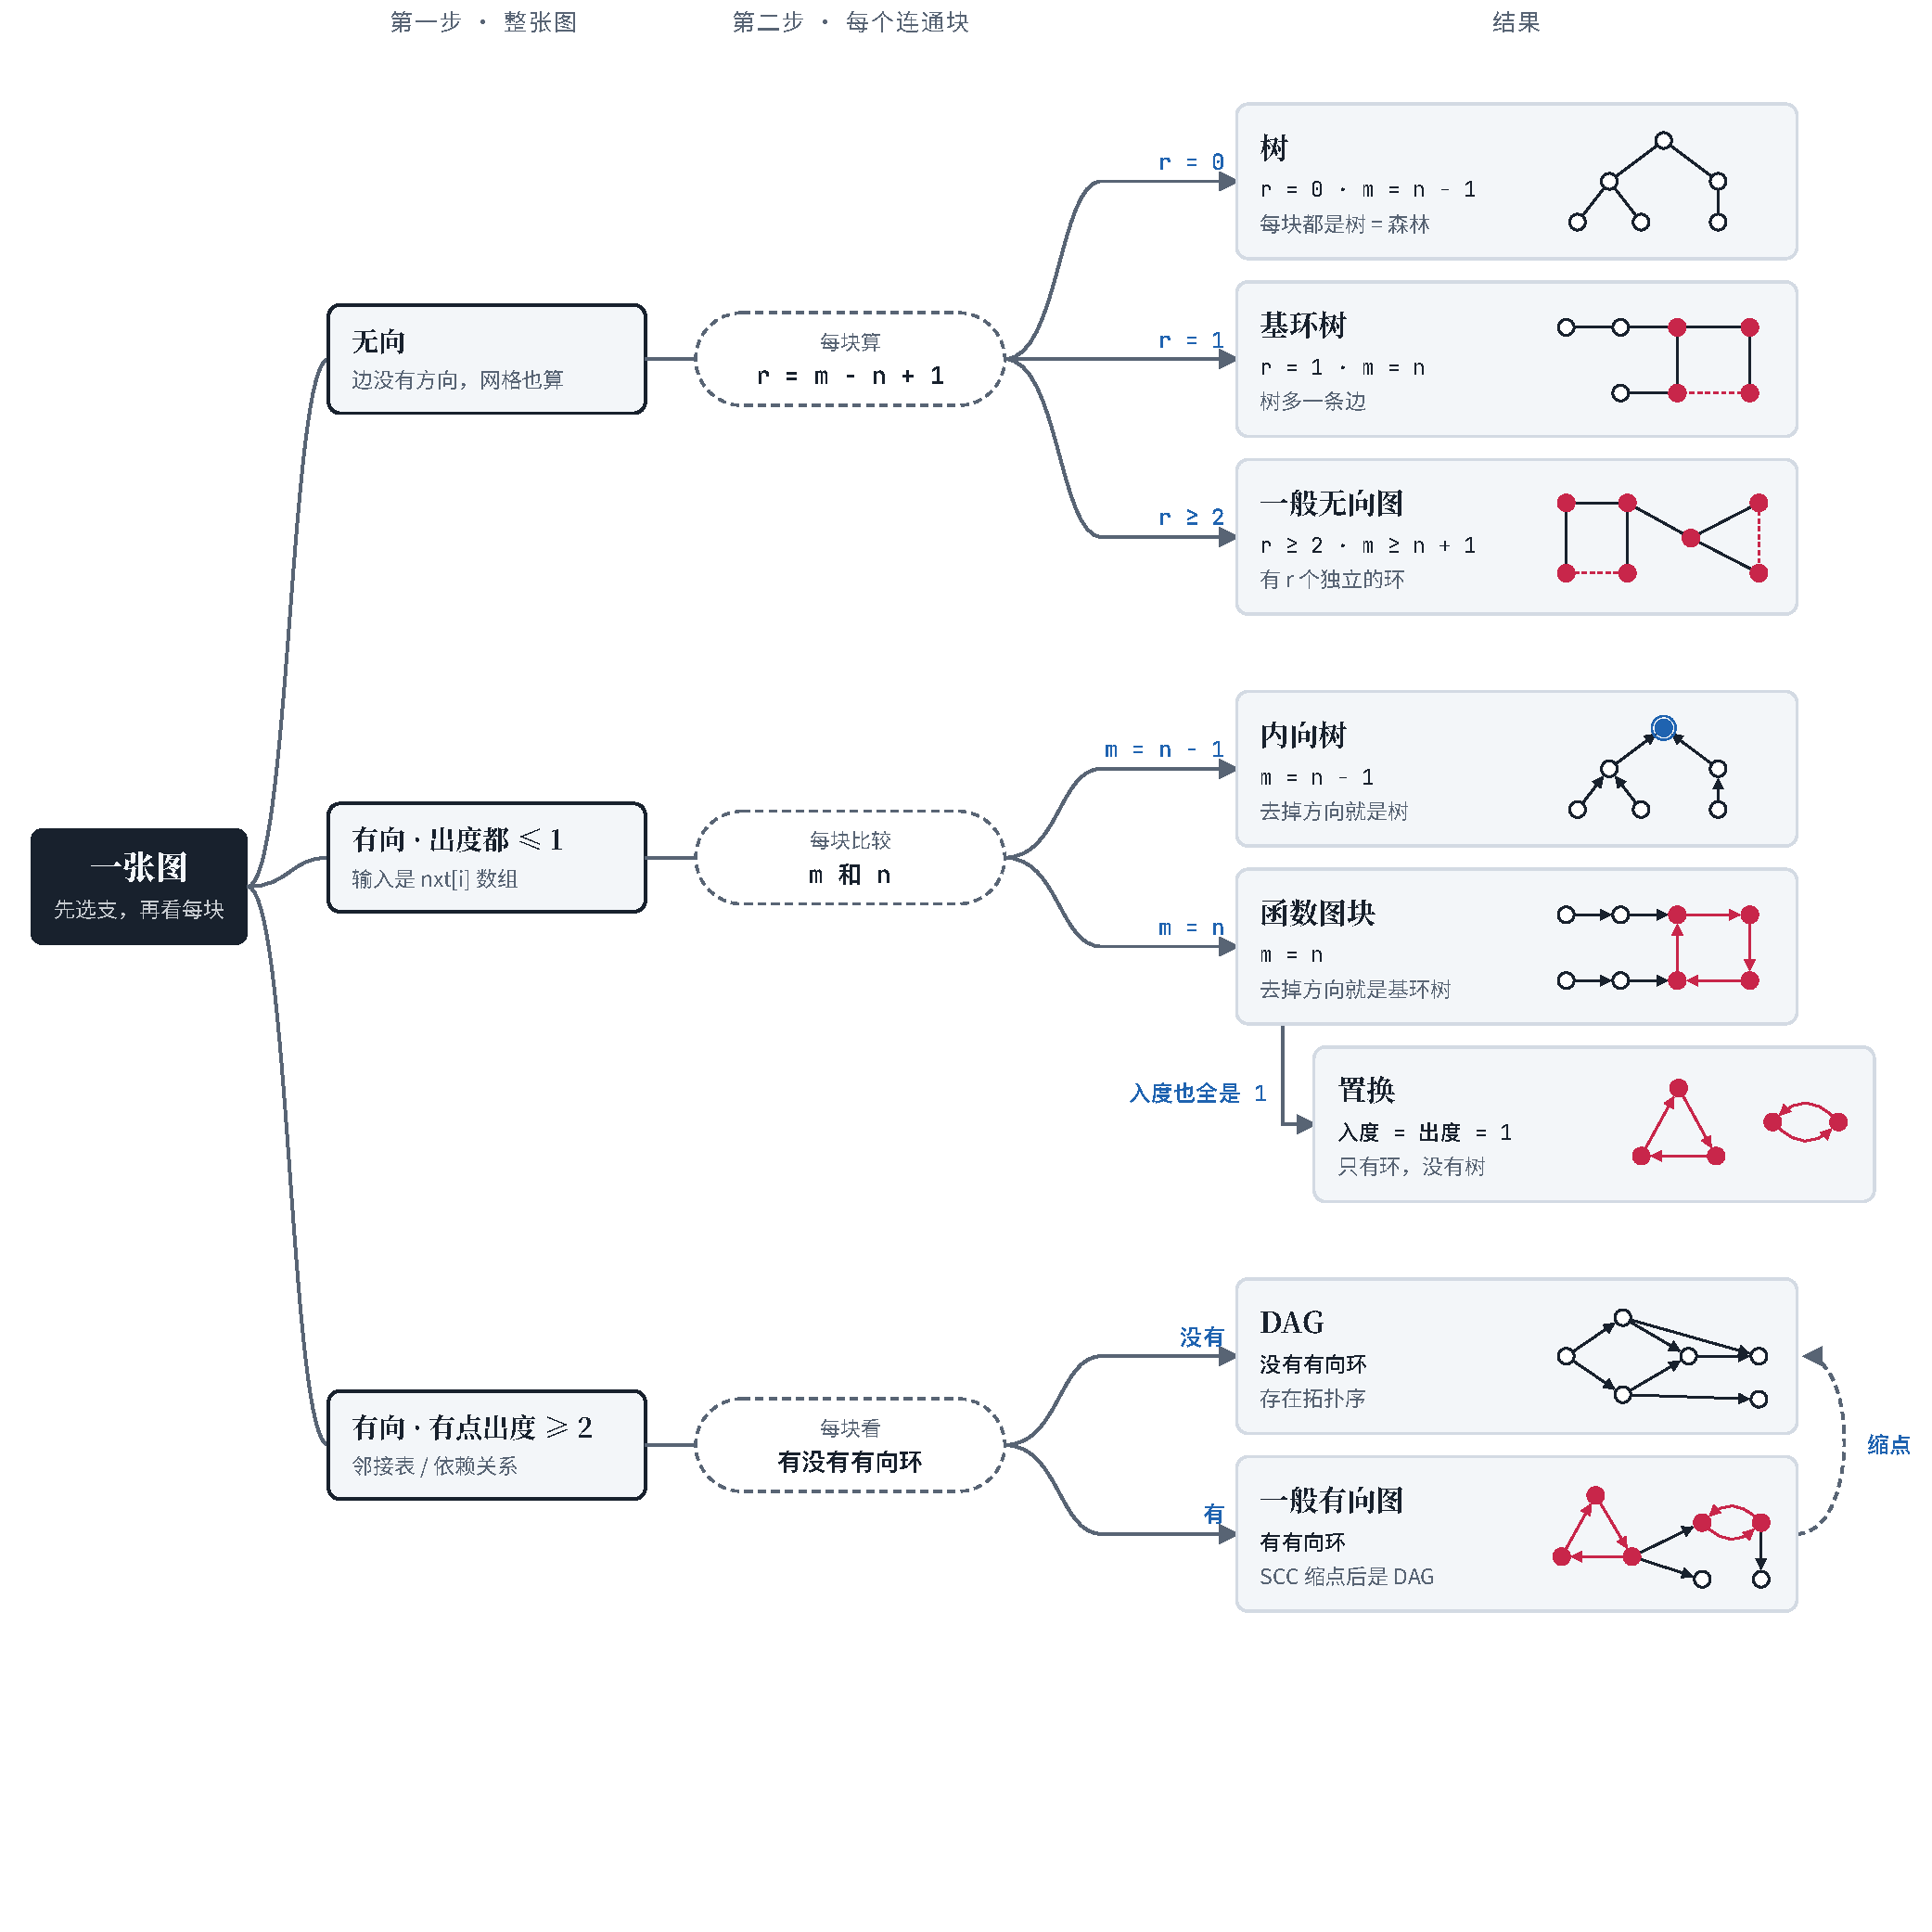
\includegraphics[width=\linewidth,trim=0 140 0 0,clip]{fig-graph-shapes.pdf}
\end{center}

记号：$n$ = 一块的点数，$m$ = 一块的边数，$r = m - n + 1$ = 一块里独立环的个数。
整张图有多个块时，第二步对每块各做一次，不同的块可以落在不同的叶子上；整张图合计的独立环数是 $m - n + c$（$c$ = 块数）。

\begin{principle}
每题三步：\textbf{判断是哪片叶子} $\to$ \textbf{这片叶子保证了什么} $\to$ \textbf{题目问的东西在环上还是在树上}（通常要分开算）。
\end{principle}

\subsection{为什么这样分}

\begin{itemize}
\item \textbf{前两支只看边数就够。}出度 $\le 1$ 时，去掉方向看到的环一定也是有向环：环上要是有个点两条环边都往外指，它的出度就是 2。
所以无向和出度 $\le 1$ 两支，数边就等于数环。
\item \textbf{出度 $\le 1$ 只有两片叶子。}有出边的点各贡献一条边，所以 $m = n - (\text{出边是 } {-1} \text{ 的点数})$。
连通至少要 $n-1$ 条边，所以出边是 $-1$ 的点最多一个：有一个是内向树，没有就是函数图块。
\item \textbf{第三支不能看边数。}$0\to1,\ 1\to2,\ 0\to2$ 去掉方向是个三角形，$m = n$，但没有有向环，是 DAG。方向会让边数失效，只能直接判有没有有向环。
\end{itemize}

\begin{principle}
$(m, n, c)$ 三个总数只能定出整张图的独立环数 $m - n + c$。环分在哪几块、有没有方向都看不出来；
只有出度 $\le 1$ 这一支能用它们把每块的类别完全定死：内向树有 $n - m$ 块，函数图块有 $m - n + c$ 块。
\end{principle}

\subsection{8 种形状}

{\small
\begin{tabularx}{\linewidth}{@{}>{\bfseries}l l X l@{}}
\toprule
\textbf{形状} & \textbf{条件（每块）} & \textbf{保证什么} & \textbf{细讲}\\
\midrule
树 & 无向，$r = 0$（$m = n-1$） & 任意两点恰好一条路径；剥度为 1 的点能剥光，最后 1–2 个点是中心 & L2 树\\
基环树 & 无向，$r = 1$（$m = n$） & 恰好一个环；多出来的边一定在环上；剥度为 1 的点剩下恰好是环 & 第 3 章\\
一般无向图 & 无向，$r \ge 2$ & $r$ 条非树边各闭上一个环；剥度为 1 的点剩下 2-core & 第 3 章\\
内向树 & 出度 $\le 1$，$m = n-1$ & 正好一个点出边是 $-1$，它是根；并查集的 parent 数组就是它 & L3 并查集\\
函数图块 & 出度 $\le 1$，$m = n$ & $\rho$ 形：正好一个有向环，树挂在环上；按入度剥叶子剩下恰好是环 & 第 4 章\\
置换 & 函数图块，入度也都是 1 & 只有环、没有树；排序最少交换次数 $= n -$ 环数 & 第 4 章\\
DAG & 有点出度 $\ge 2$，无有向环 & 存在拓扑序；按入度能剥光；沿拓扑序 DP 不会循环依赖 & 第 3、5 章\\
一般有向图 & 有点出度 $\ge 2$，有有向环 & 有环 $\Leftrightarrow$ DFS 有边指向灰点；SCC 缩点后是 DAG & 第 3 章\\
\bottomrule
\end{tabularx}
}

\subsection{\texorpdfstring{题型 $\to$ 解法 $\to$ 例题}{题型 → 解法 → 例题}}

思维导图的第三层：每片叶子下面常见的问法。例题是 LeetCode 题号。

{\small
\begin{longtable}{@{}p{0.27\linewidth} p{0.56\linewidth} p{0.11\linewidth}@{}}
\toprule
\textbf{问法} & \textbf{解法} & \textbf{例题}\\
\endhead
\midrule
\multicolumn{3}{@{}l}{\textbf{树}}\\
\quad 是不是一棵树 & m = n $-$ 1 并且连通；或者并查集一路没成环 & 261\\
\quad 最矮的根 / 中心 & 剥度为 1 的点，一层层剥，最后剩下的 1–2 个就是中心 & 310\\
\quad 直径 / 最长路径 & 两次 BFS：从任意点走到最远点 a，再从 a 走到最远点；或子树 DP 记最长的两条链 & 1245、543\\
\quad 每个点当根的答案 & 换根 DP：第一遍 DFS 算子树信息，第二遍从父亲推到孩子 & 834\\
\midrule
\multicolumn{3}{@{}l}{\textbf{基环树}}\\
\quad 哪条边是多出来的 & 并查集，第一条两端早就连通的边 & 684\\
\quad 找出环 / 点到环的距离 & 剥度为 1 的点剩下环；环上的点距离为 0，从它们一起多源 BFS & 2204\\
\quad 基环树上做 DP & 断开环上一条边，变成一棵树；断边两端分情况各做一遍树形 DP。213 是只有环、没有树的版本 & 213\\
\midrule
\multicolumn{3}{@{}l}{\textbf{一般无向图}}\\
\quad 连通块个数 / 合并 & 并查集，或每个没访问过的点 DFS 一次 & 323\\
\quad 有没有环 & 并查集：加边前两端已连通；DFS：碰到不是父亲的已访问点 & 1559\\
\quad 最短环 & 每个点做一次 BFS，非树边给出候选 dist[u] + dist[v] + 1，取最小 & 2608\\
\quad 能不能二分（有没有奇环） & BFS 染色，相邻两点同色就冲突；冲突 $\Leftrightarrow$ 有奇环 & 785\\
\quad 桥 / 割点 & Tarjan：DFS 记 dfn 和 low，看子树能不能绕非树边回到上面 & 1192\\
\midrule
\multicolumn{3}{@{}l}{\textbf{内向树}}\\
\quad 第 k 个祖先 & 倍增：up[j][v] 由两次 up[j $-$ 1] 拼出；k 按二进制位往上跳 & 1483\\
\quad 两点的最近公共祖先 & 两条往根走的链表求交点；或者先对齐深度再一起往上走 & 1650\\
\quad 每个点到根的路径和 & 沿 parent 记忆化：dist[v] = w[v] + dist[parent[v]] & 1376\\
\quad 子树聚合（大小、得分） & 建孩子表做 DFS；或按入度剥叶子，把孩子的值推给父亲 & 2049\\
\midrule
\multicolumn{3}{@{}l}{\textbf{函数图块}}\\
\quad 找环 / 最长环 & 时间戳：撞到这一轮编过号的点，环长 = 当前时钟 $-$ 它的时间戳 & 2360\\
\quad 每个点能走到几个点 / 到环的距离 & 剥叶子分开环和树；环上的点看环长，树上的点按剥的顺序倒着推 ans[u] = ans[f(u)] + 1 & 2876\\
\quad 用环和链拼答案 & 按环长分类讨论；剥叶子时顺手记进每个点的最长链 & 2127\\
\quad 走 k 步，k 很大 & 倍增；或者算出尾巴 + 整圈数 + 余数 & 2836\\
\quad 单个起点的入环点 & Floyd 快慢指针：相遇后一个回起点，两个同速走，再相遇的点就是入环点 & 287、142\\
\quad 两个起点的最近汇合点 & 从两个起点各走一遍记 dist（只有一条路），再挑 max 最小的点 & 2359\\
\midrule
\multicolumn{3}{@{}l}{\textbf{置换}}\\
\quad 排序最少交换几次 & 当前位置指向排好序后的位置，答案 = n $-$ 环数 & 2471\\
\quad 原地归位 / 找缺失的数 & 环排序：把 x 一路换到它该在的位置 & 41、448\\
\quad 重复几次回到原样 & 每个环各转各的，周期 = 各环长的 lcm & 1806\\
\midrule
\multicolumn{3}{@{}l}{\textbf{DAG}}\\
\quad 排出一个顺序 & Kahn：入度为 0 的点入队，剥出来的顺序就是拓扑序 & 210、2392\\
\quad 最长路径 / 路径计数 & 沿拓扑序 DP，每个点的值由所有前驱推出来 & 2050、1857\\
\quad 谁是谁的前置（传递关系） & 沿拓扑序把每个点的前置集合传给后继 & 1462\\
\quad 网格里严格单调地走 & 边从小指向大，天然无环，是隐式 DAG；记忆化 DFS 即可 & 329\\
\midrule
\multicolumn{3}{@{}l}{\textbf{一般有向图}}\\
\quad 有没有环 / 能不能全部完成 & Kahn 剥不完就有环；或三色 DFS 碰到指向灰点的边 & 207\\
\quad 哪些点永远走不进环 & 建反图，按出度剥，能剥掉的就是 & 802\\
\quad 有向最短环 & 每个点 BFS，第一条指回起点的边 u $\to$ s 给出 dist[u] + 1 & —\\
\quad 环上的点要当成一个整体 & SCC 缩点后变成 DAG，再套 DAG 的题型。LC 少见，CF 常见 & —\\
\bottomrule
\end{longtable}
}

\subsection{两条统一规律}

\textbf{剥叶子：剩下的是什么。}反复删掉入度为 0（或度为 1）的点，删不掉的那部分只和环有关。

{\small
\begin{tabularx}{\linewidth}{@{}l X X l@{}}
\toprule
\textbf{怎么剥} & \textbf{一般情况剩下} & \textbf{特例} & \textbf{题}\\
\midrule
有向，按入度 & 环 + 从环出发能走到的点 & DAG 剥光（顺序即拓扑序）；函数图块剩下\textbf{恰好是环} & 207、2876\\
有向，按出度（反图） & 环 + 能走进环的点 & 剥掉的点 = 永远走不进环的点 & 802\\
无向，按度 = 1 & 2-core：环和连接环的路 & 树剥光（最后 1–2 个点是中心）；基环树剩下\textbf{恰好是环} & 310、2204\\
\bottomrule
\end{tabularx}
}

\textbf{遍历：哪种边闭上环。}DFS / BFS 都会长出一棵树，环一定来自非树边。不同叶子的差别只在于哪种非树边算数。

{\small
\begin{tabularx}{\linewidth}{@{}l X X l@{}}
\toprule
\textbf{形状} & \textbf{算环的边} & \textbf{要记的状态} & \textbf{题}\\
\midrule
无向 / 网格 & 任何不回父亲的非树边 & 来过没有 + 父亲，或直接并查集 & 684、1559\\
无向，求最短环 & 同上，候选 \code{dist[u]+dist[v]+1} & 每个起点一次 BFS & 2608\\
一般有向 & 指向\textbf{灰点}的边；指向黑点的不算 & 三色：白 / 灰 / 黑 & 207\\
出度 $\le 1$ & 指向这一轮编过号的点 & 时间戳 + \code{round\_begin}（三色的特化） & 2360\\
\bottomrule
\end{tabularx}
}

走 $k$ 步的倍增是第 1 章快速幂那条线，只是题目出在函数图上（第 4 章）。
